\documentclass{article} % For LaTeX2e
\usepackage{nips13submit_e,times}
\usepackage{hyperref}
\usepackage{url}
\usepackage{verbatim}
\usepackage{graphicx}
\usepackage{subcaption}
\usepackage{listings}
\usepackage{clrscode4e}
\usepackage{tikz}
\usepackage{amsmath}


%\documentstyle[nips13submit_09,times,art10]{article} % For LaTeX 2.09


\title{Incremental Construction of Programs in a Multitask Setting}

% \begin{comment}
\author{
Kevin Ellis\thanks{Questions and correspondence should be sent to 
\href{mailto:ellisk@mit.edu}{ellisk@mit.edu}.} \\
Department of Brain \& Cognitive Sciences\\
MIT\\
\And
Eyal Dechter \\
Department of Brain \& Cognitive Sciences\\
MIT\\
\AND
Ryan P. Adams \\
School of Engineering \& Applied Sciences \\
Harvard University\\
\And
Joshua B. Tenenebaum \\
Department of Brain \& Cognitive Sciences\\
MIT\\
}
% \end{comment}
% The \author macro works with any number of authors. There are two commands
% used to separate the names and addresses of multiple authors: \And and \AND.
%
% Using \And between authors leaves it to \LaTeX{} to determine where to break
% the lines. Using \AND forces a linebreak at that point. So, if \LaTeX{}
% puts 3 of 4 authors names on the first line, and the last on the second
% line, try using \AND instead of \And before the third author name.

\newcommand{\fix}{\marginpar{FIX}}
\newcommand{\new}{\marginpar{NEW}}

\nipsfinalcopy % Uncomment for camera-ready version

\begin{document}


\maketitle

\begin{abstract}
How can machine learning techniques be used to solve problems whose solutions are best represented as computer programs? For example, suppose a researcher wants to design a probabilistic graphical model for a novel domain. Searching the space of probabilistic models automatically is notoriously difficult and is especially difficult when the latent variables are possible. However, when researchers seem able to relatively easily adapt commonly used modeling motifs to new domains. In doing so, they draw on abstractions such as trees, chains, grids and plates to constrain and direct the kinds of models they produce. This suggests that before we ask machine learning algorithms to discover parsimonious models of new domains, we should develop techniques that enable our algorithms to automatically learn these ``graphical concepts'' in much the same way that researchers themselves do, by seeing examples in the literature. One natural way to think of these graphical concepts is as programs that take sets of random variables and produce graphical models that relate them. In this work, we describe the SEC algorithm, which attempts to learn a distribution over programs by incrementally finding program components that commonly help to solve problems in a given domain, and we show prelimarily that SEC is able to discover the graphical concepts that underlie many of the common graphical model structures.  
\end{abstract}


\section{Introduction}


The vast majority of research in machine learning is focused on utilizing large amounts of noisy data living in high-dimensional, real-valued vector spaces. Such research has been immensely successful and has enabled automatic and accurate modelling on a scale that was previously infeasible. However, when we want to build a car, draw a painting, or design the machine learning models to which we apply our new algorithms and techniques, we face problems that current machine learning tools are unable to handle. The highly structured objects that humans produce seems to require a different representation than the ones which machine learning algorithms have most successfully employed. 

One example of a structured representation we would like to be able to learn is the probabilistic graphical model. Although graphical models are widely used in machine learning to represent the factorizes structure of probability distributions, they are generally designed by researchers rather than by algorithms. This is especially true when the goal is to learn about latent variables underlying the observed data, because it is difficult to capture the knowledge which allows researchers to make reasonable assumptions about which latent variables exists and what they depend on. 

In particular, machine learning researchers make frequent use of graphical motifs and abstractions such as trees, chains, rings, grids, mixtures, and plates to constrain the space of graphical models they consider. But how do they learn that these are good motifs? How do they learn how to use them and combine them to design new models? 

One hypothesis is that these motifs and abstractions are best represented as programs that manipulate and compose graph operations. In this work, we discuss how one could learn these motifs and abstracts by finding programs that generate commonly occured graphical model types. In particular, we present the SEC algorithm, a general purpose multitask program induction algorithm, that attempts to solve many related tasks by generating a weighted library of useful subroutines that induces a distribution over the space of programs. We discuss how SEC can be used to extract from a set of training tasks the kind of abstract knowledge that machine learning researchers bring to the task of designing graphical models, and we speculate that learning such representations can assist in the difficult tasks of automatically finding good latent-variable graphical models for novel datasets. 

% To address this problem, many structured representations have been proposed in the machine learning and AI literatures: learning over graphs \cite{}, grammars\cite{}, Horn clauses\cite{}, relations{}, etc., has been investigated. These are representations that attempt to bridge the gap between the tractablity of learning and reasoning in smooth continuous spaces and the expressivity of general purpose programming languages. 

% However, many of the most natural representations of structured domains are best described as programs and are difficult to fit into more restrictive representations.  To take an example directly from the machine learning literature, consider the plate notation~\cite{DBLP:journals/jair/Buntine94} commonly used to describe graphical models over collections of variables. A typical example is shown in Figure~\ref{fig:lda_plate}~\cite{DBLP:journals/jmlr/BleiNJ03}. The goal of plate notation is precisely to express the notion of a ``for loop'' within the graphical model representation. One reason this is a convenient tool is that researchers conceptualize their models as sampling procedures -- easily expressed as programs (see Figure~\ref{fig:lda_code}, but not as static graphs -- and can use plate notation to express a commonly occuring control structure. In fact, the field of probabilistic programming, which has gained recent popularity, is spurred on by exactly the motivation that our models are most naturally expressed as programs. 

% Suppose, then, that we want to create machine learning algorithms that can help discover good models for data in novel domains; that is, we want algorithms that discovers the structure of the latent graphical model underlying the data. This is a field of active research \ 

% In this paper, we describe our approach to learning over structured representations as a search over the space of programs in a functional programming language. We characterize learning in this space as incrementally building a weighted library of program abstractions, i.e. a collection of subroutines, that are commonly used to solve problems in a given domain. The SEC algorithm (for Sequential Exploration-Compression), which we present here, takes a set of related tasks and produces a distribution over programs that solve those tasks; as it refines this distribution, SEC is able to search the space of programs more efficiently and solve more tasks. 

% We will present here two domains of interest. First, continuing with the example above, we will describe how SEC can learn to efficiently explore the space of relevant graphical models for a given problem. Second, we will examine SEC's performance on a completely different type of task, in which we want to an algorithm to build tall and physically stable block towers. 

% \lstset{
% 	basicstyle=\scriptsize\ttfamily,
%     commentstyle=\color{white!40!black},
%     escapechar=+,
%     escapebegin=\color{white!40!black},
%     escapeend={},
%     keywordstyle=\bfseries\color{Periwinkle},
%     numbers=left,
%     numberstyle=\sffamily\tiny\color{gray},
% }


% \begin{figure}[h]
% \centering
% \begin{subfigure}{.5\textwidth}
%   \centering
% 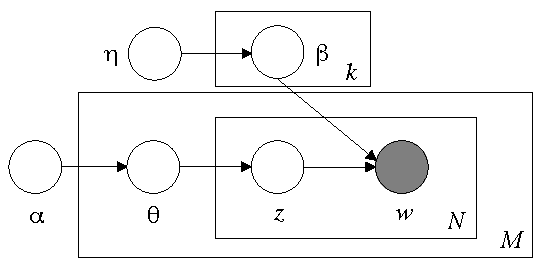
\includegraphics[width=.7\linewidth]{./figures/lda_plate_blei.pdf}
%   \caption{An example of typical plate notation use. \label{fig:lda_plate}}

% \end{subfigure}%
% \begin{subfigure}{.4\textwidth}
% 	\begin{lstlisting}[frame=single, numbers=none, xleftmargin=0pt]
% 	for +$k$+ = 1:NumTopics
% 	  +$\beta$+[k] +$\sim$+ Dirichlet(+$\eta$+)
% 	for m = 1:NumDocuments
% 	  +$\theta$+[m] +$\sim$+ Dirichlet(+$\alpha$+) 
% 	  for n = 1:NumWords 
% 	    z +$\sim$+ Categorical(+$\theta$+[m])
% 	    w+$\sim$+ Categorical(+$\beta$+[z])
% 	\end{lstlisting}
%   \caption{The same model as a program.}
%   \label{fig:lda_code}
% \end{subfigure}
% \caption{The popular Latent Dirichlet Allocation model in two forms.}
% \label{fig:lda}
% \end{figure}


\section{The SEC Algorithm}

The SEC algorithm takes a library of primitives and a set of related tasks to solve; its goal is to produce a set of programs that solve these tasks. Like the EC algorithm~\cite{DBLP:conf/ijcai/DechterMAT13}, of which it an extension, the SEC algorithm maintains a distribution $\mathcal{D}$ over programs. This distribution helps guide its search to relevant parts of of the space of programs. In each iteration, SEC does two things: first, it uses $\mathcal{D}$ to explore the space of programs that are likely to be relevant for the tasks it has been given; and second, compresses the solutions it found and uses this compression generate a new weighted library of primitives that defines an updated $\mathcal{D}$.


\subsection{Generative Model}
The SEC algorithm can be expressed as MAP inference in a probabilistic generative model over the space of programs that captures two intuitions: 1) for a set of related tasks, useful programs are composed of useful subparts, and 2) short programs are a priori more likely than long programs. 

Our generative model assumes that the programs that solve a set of related tasks are themselves constructing by composing program fragments that are drawn from a common stochastic grammar. This grammar is itself drawn from a distribution over grammars that is biased towards grammars with smaller descriptions lengths. This generative model is shown in Figure~\ref{ref:gm}.

\begin{figure}
\begin{codebox}
\li \id{G} $\sim$ $P_G(\cdot)$ \Comment{Draw grammar from description-length prior}
\li \id{\ell_n} $\sim\mbox{Uniform}(1, L)$ \Comment{Draw number of subprograms in $n^{th}$ program}
\li \Comment{Draw $\rho_n$, the $n^{th}$ program, by composing its subprograms, $e_n^{i}$}
\li \id{e_n^{i}} $\sim P_{e|G}(\cdot | G)$
\li \id{\rho_n} $= e_n^{\ell_n} (e_n^{\ell_n-1} ( \cdots e_n^{1}))$
\li \Comment{Draw $t_n$ by adding noise $\epsilon_n$ to the output of $\rho_n$}
\li \id{\epsilon_n} $\sim P_{\mbox{noise}}(\cdot)$
\li \id{t_n} $= \rho_n + \epsilon_n$
\end{codebox}
\caption{The generative model underlying the SEC algorithm. \label{ref:gm}}
\end{figure}

\subsection{Inference}
We implement an version of the EM algorithm~\cite{dempster:1977} for MAP estimation of the grammar, $G$, given the tasks, $\{t_n\}$. The hidden data in this case is the latent program that solves each task.

The joint distribution factorizes as
\begin{equation}
P(G,\{\rho_n\},\{t_n\}) = \frac{1}{L^N} P(G) \prod_n P(t_n | \rho_n) P(\rho_n | G),
\label{eq:joint}
\end{equation}
where $P(\rho_n | G) = \prod_i P(e^i_n | G)$.
From equation (\ref{eq:joint}), the EM updates are
\begin{eqnarray}
q(\rho_n) &\propto& P(t_n | \rho_n) P(\rho_n | G^{\text{old}})\\
\label{eq:qdist}
G^{\text{new}} &=& \operatorname{argmin}_G \left( -\ln P(G) -
\sum_n 
E_{q_n}
 \left[ \ln P(\rho_n | G) \right] \right)
 \label{eq:gmax}
\end{eqnarray}

Exact computation of the normalizing constant in equation (\ref{eq:qdist}), or the expectation in equation (\ref{eqn:gmax}), would require summing over the infinite space of programs that can be generated from the grammar. To approximate this expectation, we perform a heuristic search over the space of programs, with the goal of finding those programs for which $q(\cdot)$ is high.
%Rather than use mutation and crossover operators, as done in genetic programming, or random resampling of subprograms, as done in recent work in applying Metropolis-Hastings to program learning, we propose that the search moves should themselves be programs drawn from the grammar $G$.
Concretely, in order to modify a program $e$ to produce new candidate programs, we draw a new function from our grammar, $e'$, and apply that new function to produce the program $e'(e)$.
Thus, we use the grammar not only as a distribution over programs of interest, but also as a distribution over programs that take as input other programs.

In our experiments, we used beam search. The objective function was the unnormalized posterior $P_{t_n|\rho_n}(t_n | \cdot )P_{\rho_n | G}(\cdot | G)$.
The beam was initialized to be the programs with the highest prior probability according to the grammar $G$.
Similarly, the search moves considered were those functions with the most highest prior probability under $G$.

Equation (\ref{eq:gmax}) has a natural interpretation as a form of compression.
Interpreting negative log probabilities as description lengths, the update (\ref{eq:gmax}) picks the grammar minimizing the sum of the description length of the grammar, plus the expected description length of the programs found to solve the tasks.

Performing the minimization operation in equation (\ref{eq:gmax}) is generally difficult.
We approximate the description length of the grammar by the number of unique program fragments in the grammar, multiplied by a regularization constant.
The description length of a program is approximated by the number of (not necessarily unique) program fragments in its smallest parse tree given the grammar.
A slight generalization of the Neville-Manning algorithm then permits tractible approximate maximization of (\ref{eq:gmax}).
Estimation of the production probabilities of $G$ is performed as in \cite{ijcai}.

\subsection{Program Representation}

Following~\cite{DBLP:conf/ijcai/DechterMAT13} and~\cite{DBLP:conf/icml/LiangJK10}, we use a
simply typed combinatory calculus -- a variable-free subset of the
polymorphic simply-typed lambda calculus~\cite{DBLP:books/daglib/0005958} -- as our
program representation language. The simplicity the combinatory calculus makes describing a distribution over its expressions particularly simple. A more detailed explanation and discussion of this program representation can be found in the papers cited above. 

\section{Learning to Construct Graphical Models}

Learning the structure of graphical models that capture the independencies underlying a dataset is an active area of research\cite{adams-wallach-ghahramani-2010a}\cite{ISI:000240797500002}\cite{ISI:000178037200004}\cite{ISI:A1995RX35400001}. Graphical model structures enforce the conditional independences a modeler believes exists among latent and observed random variables\cite{DBLP:books/daglib/0066829}.
In practice, the sorts of graphical models that humans design, such as Hidden Markov Models, phylogenetic trees, topic models, and Ising models, exhibit certain symmetries and recursive structures that might be amenable to synthesis by programs.

\begin{figure}[h]
% \centering
\begin{minipage}[t]{.4\textwidth}
% \vspace{0pt}
% \begin{subfigure}{.45\textwidth}
  % \vspace*{\fill}
  % \centering
  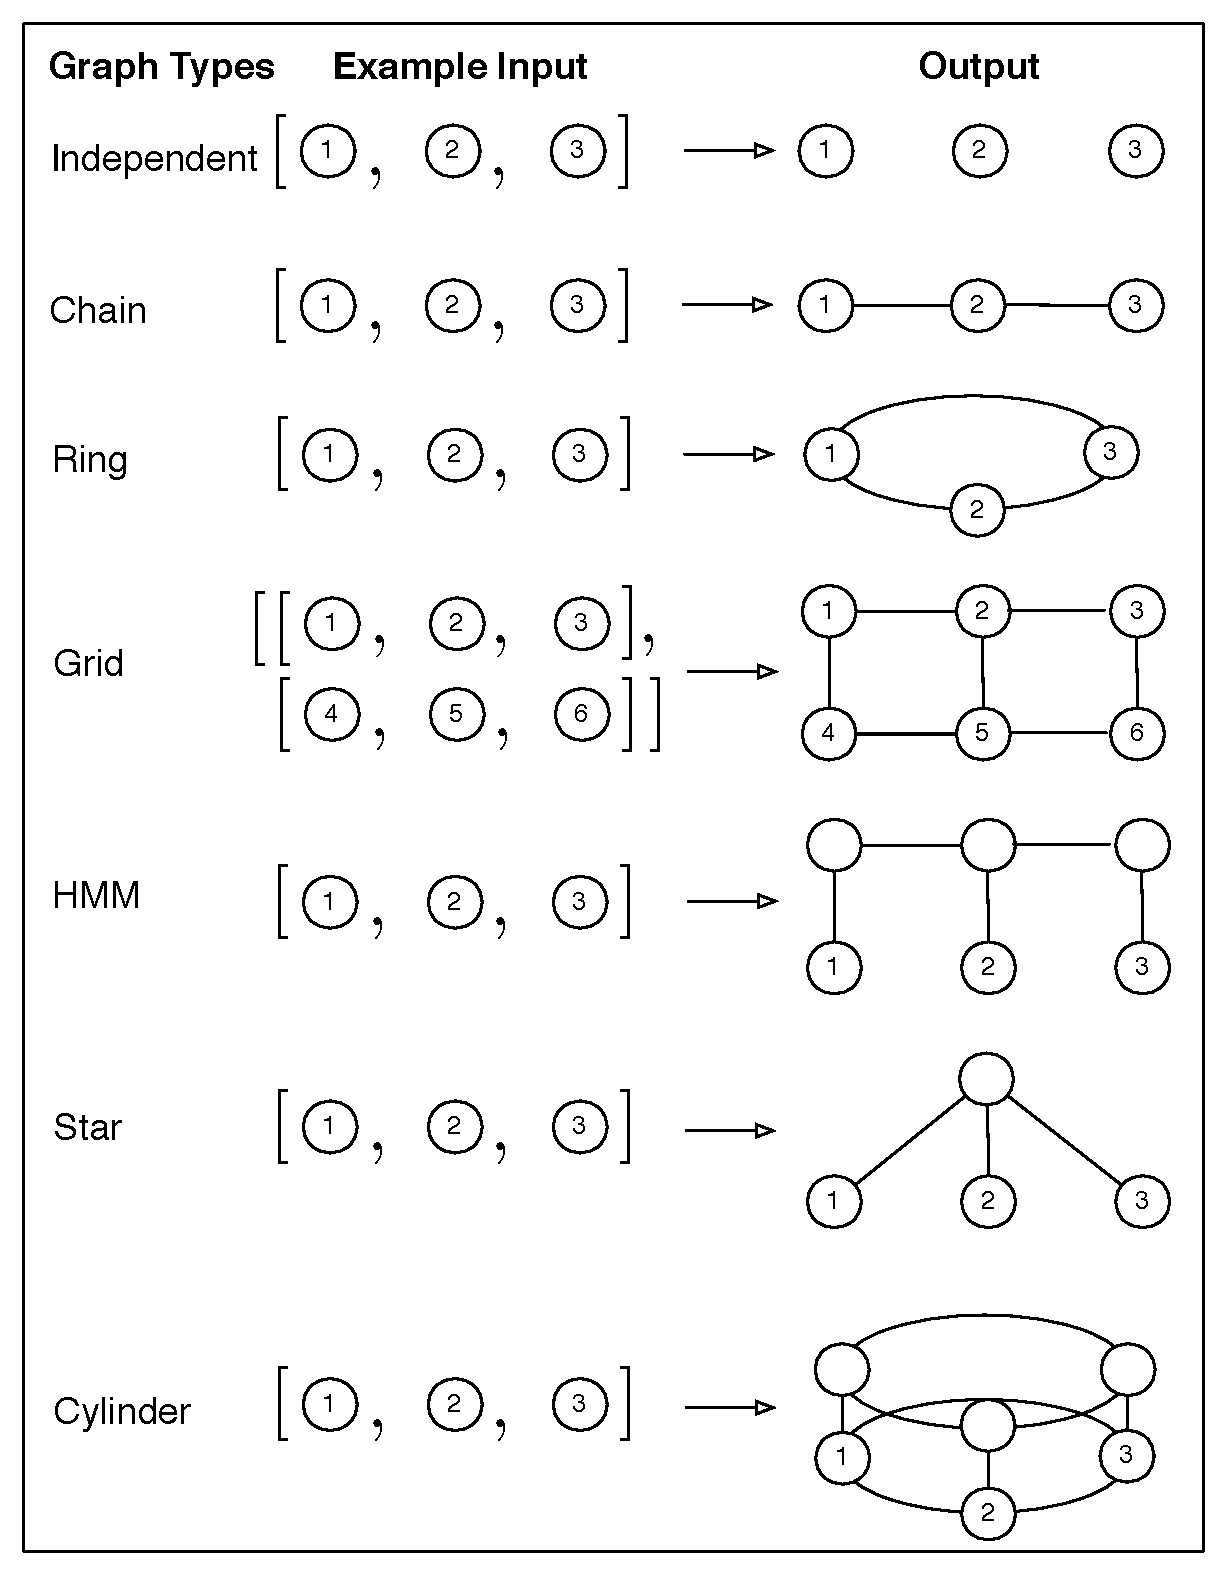
\includegraphics[width=\linewidth]{./figures/tasks.pdf}
  \caption{Example input/output pairs of learned programs. Each induced program takes as input a list of observed nodes and produces an undirected graphical model. Here, we show each program with a small number of input nodes, but the learned programs transfer arbitrary length lists of visible nodes into the corresponding graphs. Labeled nodes correspond to observed variables; unlabeled nodes correspond to latent variables.}
  \label{fig:tasks}
\end{minipage}
\hspace{1cm}
\begin{minipage}[t]{.5\textwidth}
% \vspace{\fill}
  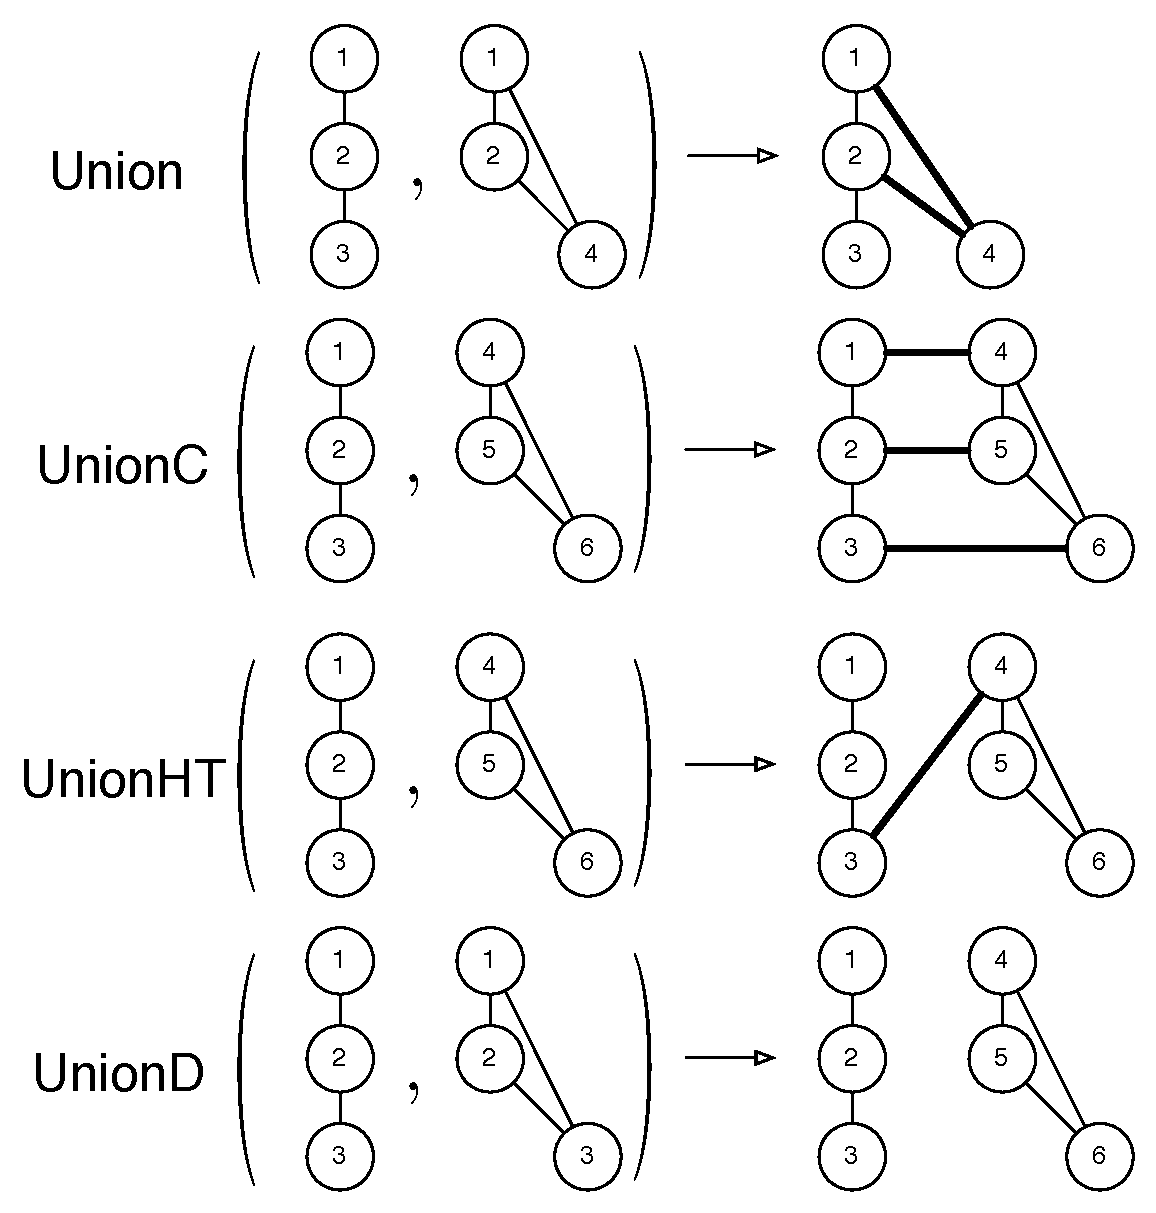
\includegraphics[width=\linewidth]{./figures/GraphCombinators.pdf}
  \caption{The operation of the undirected unions. Union: computes union of vertexes and edges. UnionC: adds edges between corresponding vertexes. UnionHT: adds edge between first (head) vertex and last (tail) vertex. UnionD: relabels input graph vertices so that they do not overlap and then computes union.}
  \label{fig:graphcomb}\par\vfill
% \end{subfigure}
\end{minipage}
\end{figure}

\subsection{Experiment}

We wanted to use the SEC algorithm to learn the common abstractions and motifs that underlie the graphical models that are commonly found in the machine learning literature. To that end, we supplied SEC with a set of twelve tasks, each of which corresponds to learning how to build a specific type of graphical model, potentially with latent vertices, given that it is provided with a list of observed verticies. A partial list of the tasks is shown in Figure~\ref{fig:tasks}. For example, the \textsc{Cylinder} task requires EC to build a program that takes as input a list of observed vertices (of any length) and produces a graph where one ring consists of the observed vertices and the other consists of corresponding latent variables. 
Tasks were specified via a set of input/output test cases, and we defined the likelihood of a program for a task to be the fraction of test cases it passed. 

The SEC algorithm was provided with an initial library of primitive  combinators, which included the basis combinators of the combinatory calculus, function list operations such as \textsc{Map} and \textsc{Foldr}/\textsc{Foldl}. We also included four binary operations on undirected graphical models, each of which computes some kind of union between two graphs. These graph operations are diagrammed in Figure~\ref{fig:graphcomb}.

%The initial library of primitive combinators contains four binary operations upon undirected graphical models.
%Each of these operations we introduce, called an \emph{undirected union}, serves to combine two smaller models while also introducing new edges.
%Using this representation, many models may be expressed in a compositional fashion when combined with higher-order combinators taken from functional programming languages, such as \emph{map} and \emph{fold}.
%The operation of these four undirected unions is diagrammed in figure (\ref{fig:graphcomb}).
%In this representation of graphs, the vertexes are given unique indexes.
%Some of the undirected unions exploit these indexes by adding edges as a function of index.



\subsection{Results}

We ran the SEC algorithm on the set of twelve tasks. The algorithm is parameterized by the frontier size, the number of unique subprograms $\{e_i\}$ enumerated from the library on each iteration. We ran the algorithm both for frontier sizes of 1000 and 5000. Note that because proposed solutions are compositions of these programs, the algorithm looks at many more potential solutions than the number of programs in the frontier. 

With a frontier size of 1000, the algorithm solves 7/12 tasks. With a frontier size of 5000, the algorithm solves 8/12 tasks. In each case, the algorithm returns solutions that partially satisfy the remaining tasks. As an example, we show in Figure~\ref{ref:cylinder} an instance of SEC's solution to the \textsc{Cylinder} task. 

Initially, SEC is unable to find solutions to the complicated graph structure tasks, such as the Ising Model or the Hidden Markov Model, even after enumerating 4 million programs through its heuristic search.
However, it is able to find programs that generate simpler graphical models, such as Markov chains.
By compressing the solutions to these simpler problems, it modifies its search procedure and, in subsequent iterations, learns more successful programs.

\begin{figure}
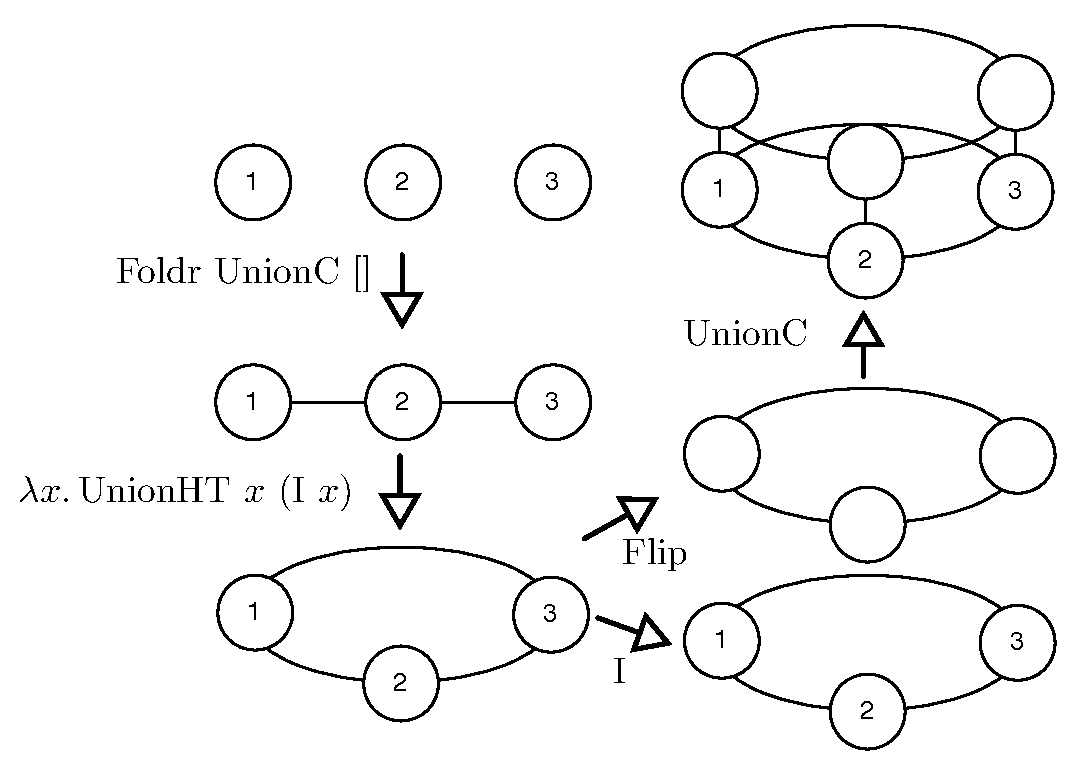
\includegraphics[width=.5\linewidth]{./figures/cylinder.pdf}
\caption{An example of how the \textsc{Cylinder} task is solved by SEC, with the basis combinators replaced by control flow arrows. The full program is written in the combinatory calculus below the image. \label{ref:cylinder}}
\end{figure}

What grammars does SEC learn, and how do they enable the bootstrap learning of more complicated programs?
The simplest example is that of how the Markov chain bootstraps the learning of the Ising model.
%Most of the easy tasks, such as the Markov chain, can be solved with the right choice of one higher-order function and one undirected union.
After one iteration, the program fragment \verb|(foldr unionC)|, used in the Markov chain program, is incorporated in to the grammar.
On the second iteration, the Ising model is learned using this fragment, producing the program \verb|(((S B) map) ((foldr unionC) null))|.

\section{Discussion}

\subsection{Relation to Prior Work}

MH sampling of programs, ILP, Kitzelman, graph grammars

\subsection{Limitations of SEC}

Does not look at data. Does everything top-down. Blind to the utility of trying one program versus another (no active learning)

\bibliographystyle{plain}
\bibliography{eyal_bib}

\end{document}
